\section{\uppercase{Proposed Method}}\label{sec:method}

\begin{figure*}[!t]\centering
  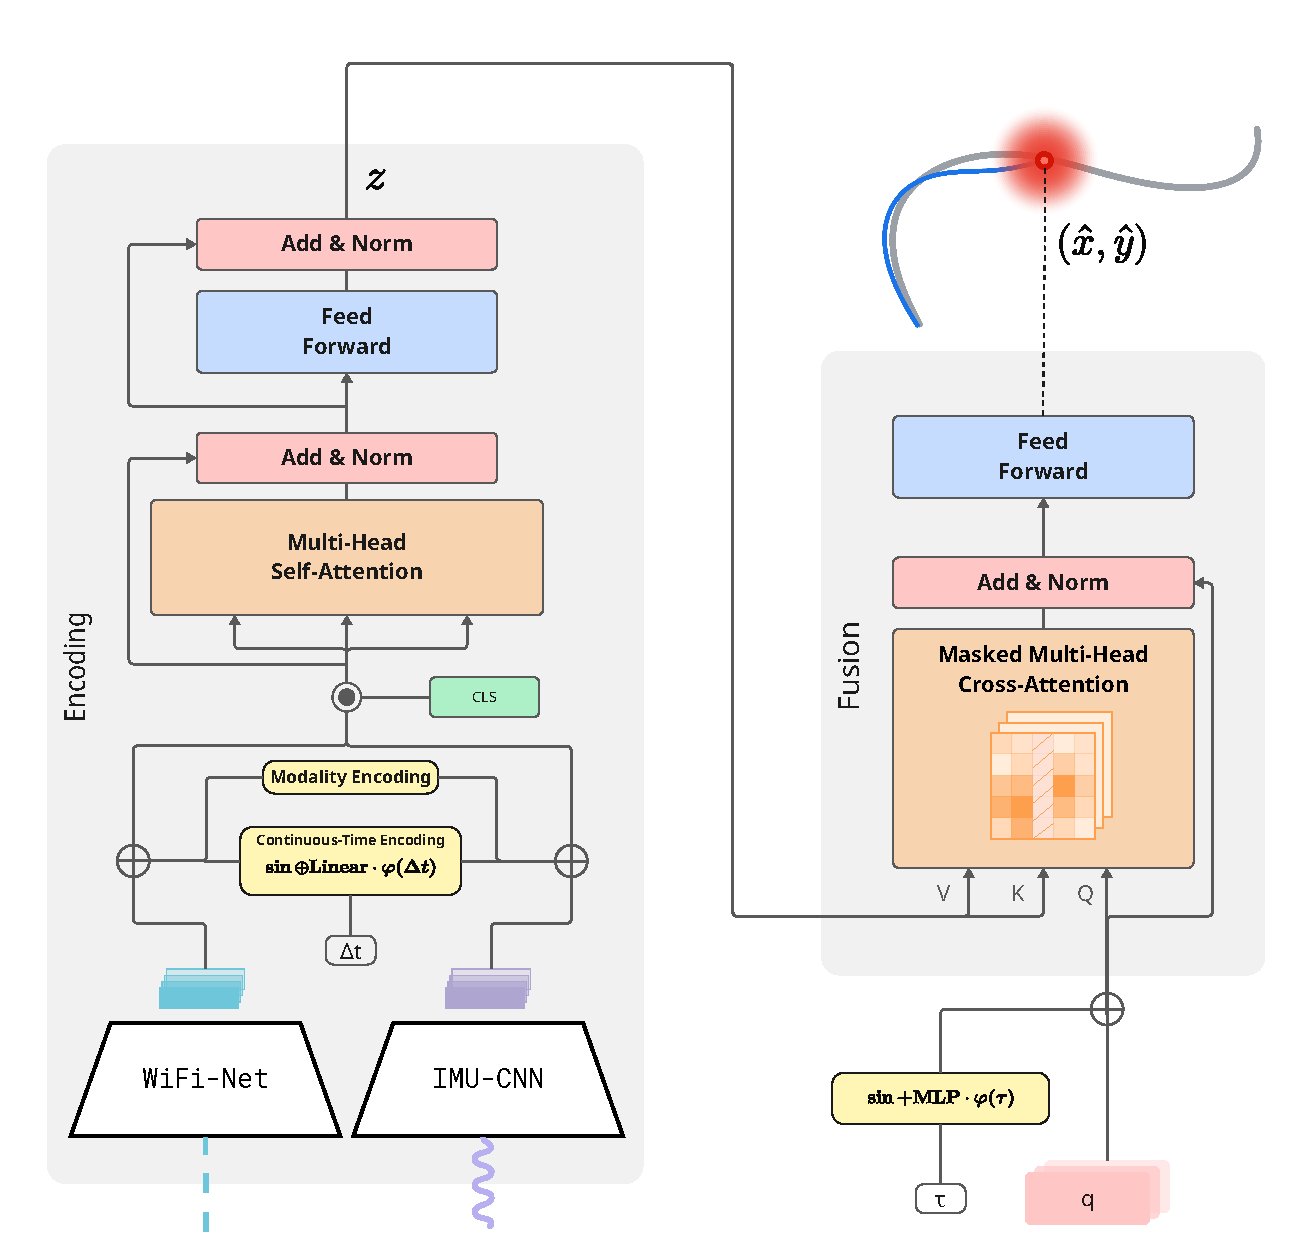
\includegraphics[width=0.9\textwidth]{figures/figure_1_latest.pdf}
  \caption{Overview of the proposed continuous-time transformer: each
    observation becomes one token, a single self-attention block fuses the set,
    and a learnable position query reads out $(\hat{x},\hat{y})$.}
  \label{fig:pipeline}
\end{figure*}

\noindent In this section, a single continuous-time set transformer is proposed to regress from the asynchronous WiFi and IMU streams to a planar position, with neither branch per modality nor resampling onto a common clock.
To this end, the problem is reformulated and analyzed in the upcoming subsections.
\subsection{Problem Reformulation and Functional Decomposition}
\noindent
In general, the absolute time instant does not influence the localization results in a relatively stable environment, but the timeliness of the data does. For localization query at instant $t_q$, the timeliness of observations $\mathcal{O}'$ is measured by the signed elapsed time
$\Delta t_i = t_i - t_q$, non-positive for a past observation. This removes $t_q$
from the inputs and casts the observations as an unordered set
\begin{equation}\label{eq:obsset}
  \mathcal{O} = \big\{\, (s_i,\, m_i,\, \Delta t_i,\, a_i) \,\big\}_{i=1}^{N},
\end{equation}
holding $K$ recent instants per modality, so $N=KM$ slots are addressable and a
slot with $a_i=0$ contributes no token. One should note that the estimate of the position depends on the sample values in set $ \mathcal{O} $ rather than the order of the samples, so the map is invariant to any
permutation $\pi$ of the set,
\begin{equation}\label{eq:perm}
  f(\pi\!\cdot\!\mathcal{O}) = f(\mathcal{O}).
\end{equation}
Because the elements of $\mathcal{O}$ differ in type, dimension and timing, $f$ is decomposed into an \emph{encoding} unit $g$ and a set-level
\emph{fusion} unit $h$, which is described as:
\begin{equation}\label{eq:decomp}
  \begin{gathered}
    f = h \circ g,\\
    g:(s_i,m_i,\Delta t_i)\mapsto \mathbf{z}_i\in\mathbb{R}^{D},\\
    h:\{\mathbf{z}_i\}\mapsto(\hat x,\hat y).
  \end{gathered}
\end{equation}

The encoding and fusion process in (\ref{eq:decomp}) can be illustrated by Figure~\ref{fig:pipeline}. Each sensor sample, whatever its rate, becomes one token of a shared latent
space, and a single self-attention block performs the entire fusion.
Figure~\ref{fig:pipeline} traces this end to end: an encoder for each modality
realizes $g$, mapping each observation to one universal token; the attention
block and a learnable position query realize $h$, which contextualizes the set
and reads out $(\hat{x},\hat{y})$.

Modality identity is carried by an additive embedding, rather than by token order; therefore, a
modality added or removed by inserting or deleting tokens brings no change to the
trunk. Tolerance to missing and stale sensors is then a property of training, without changing the architecture.


\subsection{Universal Tokenization and Encoders for Each Modality}
\label{subsec:tok}

\noindent
This section realizes the encoding $g$ of Equation~\eqref{eq:decomp}, mapping each
element of the observation set $\mathcal{O}$ to a common latent space; the fusion
$h$ that delivers the permutation invariance of Equation~\eqref{eq:perm} follows in
Section~\ref{subsec:fusion}.

The encoding $g$ sends every observation to one $D$-dimensional token holding the
measurement, its modality, and its elapsed time relative to the query,
\begin{equation}\label{eq:token}
  \mathbf{z}_i = \mathrm{enc}_{m_i}(s_i)
               + \mathbf{e}_{m_i}
               + \phi(\Delta t_i).
\end{equation}
The first term is the output of the encoder for that modality; the second a
learnable modality embedding $\mathbf{e}_m \in \mathbb{R}^{D}$, carrying sensor identity additively so it survives
permutation; the third the continuous-time encoding of $\Delta t_i$.

\paragraph{Continuous-time encoding.}
The encoding $\phi$ admits sensors of widely different rates into one model
without resampling. Unlike the discrete positional encoding of sequence
transformers, $\phi$ is a function of the real-valued $\Delta t$ in seconds. It
evaluates $n$ sinusoids whose angular frequencies $\boldsymbol{\omega} =
2\pi/\boldsymbol{\tau}$ derive from periods $\boldsymbol{\tau}$ spaced
geometrically over $[\tau_{\min},\tau_{\max}]$. Taking the sine and cosine of
each gives $2n$ features, which a learned matrix
$\mathbf{W}_\phi \in \mathbb{R}^{D \times 2n}$ projects to $D$ dimensions,
\begin{equation}\label{eq:time}
  \phi(\Delta t) = \mathbf{W}_\phi
    \big[\, \sin(\boldsymbol{\omega}\,\Delta t) \,\|\,
            \cos(\boldsymbol{\omega}\,\Delta t) \,\big].
\end{equation}
Under the geometric spacing, observation times close together receive similar
codes while distant times stay separable, across periods from $0.05$~s to
$120$~s using $n=32$ sinusoids. Reading the continuous $\Delta t$ rather than a
discrete index places every token on one shared time axis regardless of when it
arrived.

\paragraph{WiFi-Net.}
WiFi-Net encodes the modality that fixes absolute place. It treats a single RSSI
scan as a query against a learned set of $N_a$ reference points, producing a
distribution that discriminates place rather than a raw radio map. The scan
$s \in \mathbb{R}^{n_{\mathrm{ap}}}$ (Equation~\eqref{eq:spaces}) is scored against
the matrix of reference points $\mathbf{A} \in \mathbb{R}^{N_a \times n_{\mathrm{ap}}}$,
and a softmax with learned temperature $\gamma$ yields a soft assignment
$\mathbf{w}$ over the reference points,
\begin{equation}\label{eq:wifi_assign}
  \mathbf{w} = \mathrm{softmax}\!\left( \frac{\mathbf{A}\, s}{\gamma} \right)
            \in \Delta^{N_a-1},
\end{equation}
a point on the $(N_a{-}1)$-simplex. The weights $\mathbf{w}$ aggregate the
embeddings of the reference points $\mathbf{E} \in \mathbb{R}^{N_a \times D}$ into
a pooled vector, which a residual MLP with layer normalization then refines into
the token,
\begin{equation}\label{eq:wifi_token}
  \mathrm{enc}_{\mathrm{wifi}}(s) = \mathbf{t} + \mathrm{MLP}(\mathbf{t}),
  \qquad
  \mathbf{t} = \sum_{j=1}^{N_a} w_j\, \mathbf{E}_j = \mathbf{w}^{\!\top}\mathbf{E}.
\end{equation}
The reference points are learned, not tied to physical access points, so the
encoder positions them where they best discriminate place. We use $N_a=64$
reference points (Figure~\ref{fig:wifinet}).

\begin{figure}[!hb]\centering
  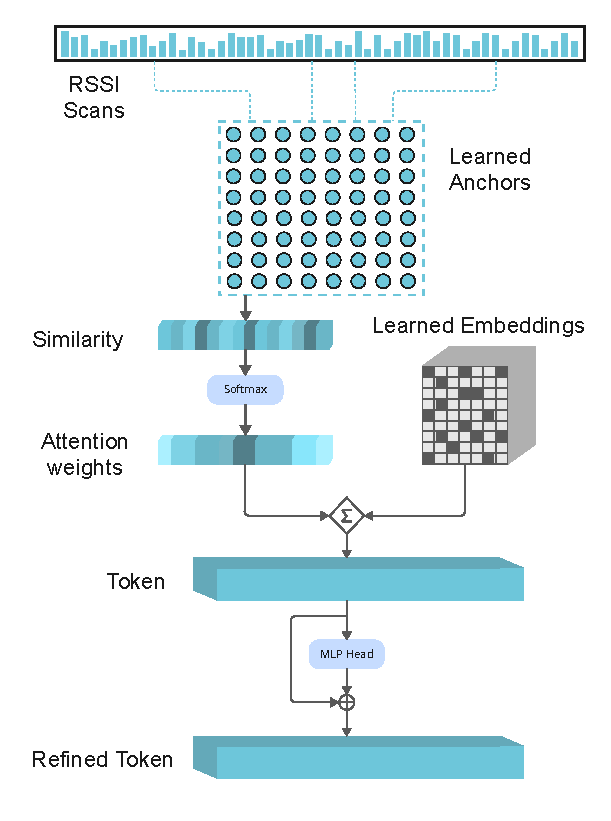
\includegraphics[width=1\columnwidth]{figures/figure_2.pdf}
  \caption{WiFi-Net encoder. An RSSI scan is scored against $N_a$ learned
    reference points; a softmax over the similarities gives attention weights that
    aggregate the learned embeddings of those reference points into a token,
    refined by a residual MLP head.}
  \label{fig:wifinet}
\end{figure}

\paragraph{IMU-CNN.}
IMU-CNN summarizes dense motion over a short temporal window, supplying the
relative motion that complements WiFi's absolute reference. The useful inertial
signature is a \emph{local} pattern in time, a brief acceleration or turn whose
contribution to position should not depend on where in the window it falls. The
encoder reads a fixed window $\mathbf{X} \in \mathbb{R}^{T \times F}$, the IMU
sample of Equation~\eqref{eq:spaces}, with $\mathbf{X}_{t,f}$ the $f$-th inertial
channel at step $t$.

The encoder is a stack of three 1D-convolutional blocks. Each block convolves a
learned filter bank along the time axis, then applies batch normalization, a
GELU nonlinearity $\sigma$ and dropout,
\begin{equation}\label{eq:imu_conv}
  \mathbf{U}^{(\ell)} = \sigma\!\big(
    \mathrm{BN}( \mathbf{W}^{(\ell)} * \mathbf{U}^{(\ell-1)} ) \big),
  \qquad \ell = 1, 2, 3,
\end{equation}
where $*$ denotes 1D convolution along time, $\mathbf{W}^{(\ell)}$ is the learned
filter bank of block $\ell$, and $\mathbf{U}^{(0)} = \mathbf{X}^{\!\top}$. Sharing
filter weights across time makes each block shift-equivariant, so a motion pattern
produces the same response wherever it falls. The three blocks raise the channel
count $F \!\to\! C_1 \!\to\! C_2 \!\to\! C_3$ and compose local responses into
deeper motion features $\mathbf{U} \equiv \mathbf{U}^{(3)} \in \mathbb{R}^{C_3
\times T'}$.

Global average pooling over time then collapses the window, averaging each
channel's response across all positions,
\begin{equation}\label{eq:imu_gap}
  \bar{\mathbf{u}} = \frac{1}{T'} \sum_{t=1}^{T'} \mathbf{U}_{:,t}
    \;\in\; \mathbb{R}^{C_3}.
\end{equation}
Pooling turns the blocks' shift-equivariance into shift-invariance: any temporal
shift of a feature leaves $\bar{\mathbf{u}}$ unchanged. A head of a linear layer
$\mathbf{W}_o$ with layer normalization sends this summary to the $D$-dimensional
token,
\begin{equation}\label{eq:imu}
  \mathrm{enc}_{\mathrm{imu}}(\mathbf{X})
    = \mathrm{LN}\!\big( \mathbf{W}_o\, \bar{\mathbf{u}} \big).
\end{equation}
The window holds $T=32$ steps of $F=9$ inertial features (triaxial acceleration,
triaxial angular rate, and roll, pitch, yaw), with channels
$(C_1,C_2,C_3)=(32,64,128)$; the learned filters capture dead reckoning over short
intervals (Figure~\ref{fig:imucnn}). Both encoders emit the same $D=128$ token
width, so each enters the fusion block without wiring specific to its modality.
IMU-CNN holds about $0.05$~M parameters.

\begin{figure}[!hb]\centering
  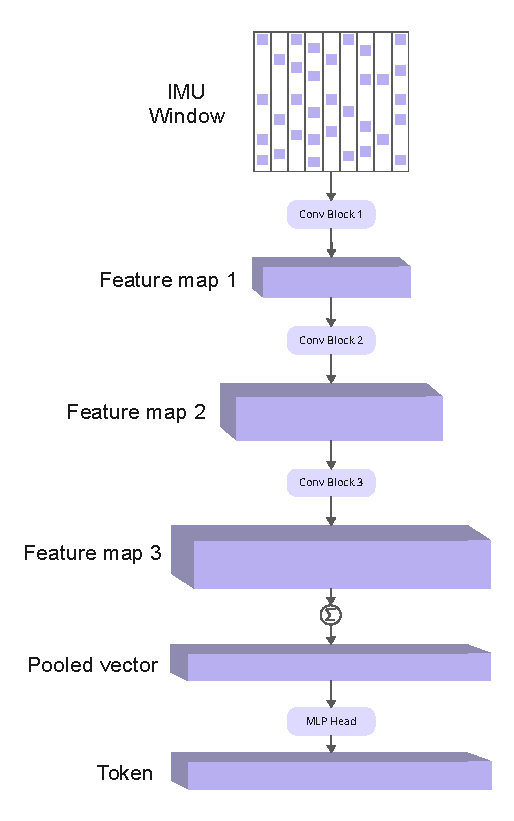
\includegraphics[width=1\columnwidth]{figures/figure_3.pdf}
  \caption{IMU-CNN encoder. A $T\times F$ inertial window passes through three
    convolutional blocks; global average pooling collapses the final feature
    map over time into a pooled vector that an MLP head maps to the token.}
  \label{fig:imucnn}
\end{figure}


\subsection{Set-Transformer Fusion and Position Readout}
\label{subsec:fusion}

\noindent
This section realizes the fusion $h$ of Equation~\eqref{eq:decomp}. The tokens of
Equation~\eqref{eq:token}, one per available observation, form the set the fusion
block aggregates. Self-attention is permutation equivariant by construction. This
is exactly the aggregation that the token encoding of Section~\ref{subsec:tok} is
built for. Once the set spans both modalities and $K$ instants, the one operation
performs cross-modal and cross-time fusion at once: a WiFi token attends to an IMU
token from a different instant exactly as to one from its own. The block stacks
$L$ pre-norm transformer encoder layers with $H$ attention heads, a feed-forward
width of $4D$ and a GELU nonlinearity. Each layer applies multi-head self-attention
(MHSA) and a position-wise feed-forward network (FFN) with residual connections,
\begin{equation}\label{eq:layer}
  \begin{aligned}
    \hat{\mathbf{Z}} &= \mathbf{Z}
      + \mathrm{MHSA}\big(\mathrm{LN}(\mathbf{Z}),\, \mathbf{B}\big), \\
    \mathbf{Z}' &= \hat{\mathbf{Z}}
      + \mathrm{FFN}\big(\mathrm{LN}(\hat{\mathbf{Z}})\big),
  \end{aligned}
\end{equation}
for a token stack $\mathbf{Z}$ and an additive padding bias $\mathbf{B}$.
Multi-head self-attention runs $H$ scaled-dot-product heads in parallel,
\begin{equation}\label{eq:mhsa}
  \mathrm{head}_h = \mathrm{softmax}\!\left(
    \frac{\mathbf{Q}_h \mathbf{K}_h^{\!\top}}{\sqrt{d_h}} + \mathbf{B}
  \right)\mathbf{V}_h,
  \quad d_h = \tfrac{D}{H},
\end{equation}
and concatenates them through an output projection. The padding bias $\mathbf{B}$
assigns $-\infty$ to every token that is absent ($a_i=0$) or dropped, so it
receives no attention mass. The set size $N$ then enters only through which tokens
are live, which is how the missing and stale conditions of
Section~\ref{sec:problem} act on the model. A learnable classification (CLS) token
is prepended and never masked, so every attention row keeps at least one live key.

The readout maps the contextualized set to a position through a single learnable
position query $\mathbf{q}$ (Figure~\ref{fig:pipeline}). The query cross-attends
to the contextualized set, with the CLS token retained in its key set, and a
two-layer MLP maps the attended vector to the predicted position
$\hat{\mathbf{p}} = (\hat{x},\hat{y})$,
\begin{equation}\label{eq:readout}
  \hat{\mathbf{p}} = \mathrm{MLP}\!\Big(
    \mathrm{CrossAttn}\big(\mathbf{q} + \phi(\tau),\; [\mathbf{c}\,\|\,\mathbf{Z}'],\; \mathbf{B}\big)
  \Big),
\end{equation}
where $\mathbf{Z}'$ is the contextualized token set, $\mathbf{c}$ the
contextualized CLS token, $\mathbf{q}$ the learnable query, and $\phi(\tau)$ the
continuous-time encoding of Equation~\eqref{eq:time} evaluated at the query offset
$\tau$, so position can be read at a chosen time. Collapsing the
permutation-equivariant set to a single output makes the full map $f$
permutation-invariant, as Equation~\eqref{eq:perm} requires.

Equation~\eqref{eq:objective-gen} poses the objective as squared error. Training
minimizes a Huber surrogate $\mathcal{H}_\delta$, quadratic for small residuals and
linear beyond a threshold $\delta$, which limits the pull of outlier positions,
\begin{equation}\label{eq:loss}
  \begin{gathered}
    \mathcal{L} = \frac{1}{N_s}\sum_{i=1}^{N_s}
      \mathcal{H}_\delta\big(\hat{\mathbf{p}}_i - \mathbf{p}_i\big),\\
    \mathcal{H}_\delta(r) =
    \begin{cases}
      \tfrac12 \lVert r\rVert^2, & \lVert r\rVert \le \delta,\\[2pt]
      \delta\big(\lVert r\rVert - \tfrac12\delta\big), & \text{otherwise,}
    \end{cases}
  \end{gathered}
\end{equation}
with $\mathbf{p}_i$ the ground truth position. The optimizer and the threshold
$\delta$ are given in Section~\ref{sec:experiments}, along with the modality and
instant dropout that confer robustness to missing and stale sensors.
Algorithm~\ref{alg:forward} assembles the encoding $g$, the fusion $h$ and the
loss into one pass.

\begin{algorithm}[!h]
\caption{Forward pass and training loss. The encoding $g$ builds the token set;
  the fusion $h$ contextualizes it and reads out the position, so
  $\hat{\mathbf{p}} = h(g(\mathcal{O})) = f(\mathcal{O})$.}\label{alg:forward}
\SetAlgoLined
\DontPrintSemicolon
\KwIn{observation set $\mathcal{O} = \{(s_i, m_i, \Delta t_i, a_i)\}$; query
  offset $\tau$; ground truth $\mathbf{p}$ (training only)}
\KwOut{prediction $\hat{\mathbf{p}} = (\hat{x},\hat{y})$; training loss $\mathcal{L}$}
\For{$i : a_i = 1$}{
  $\mathbf{z}_i \leftarrow \mathrm{enc}_{m_i}(s_i) + \mathbf{e}_{m_i}
    + \phi(\Delta t_i)$ \tcp*{encoding $g$, Eq.~\eqref{eq:token}}
}
$\mathbf{Z} \leftarrow [\,\mathbf{c}_{\mathrm{cls}} \,\|\,
  \{\mathbf{z}_i : a_i = 1\}\,]$ \tcp*{CLS never masked}
\For{$\ell \leftarrow 1$ \KwTo $L$}{
  $\mathbf{Z} \leftarrow \mathrm{Layer}_\ell(\mathbf{Z}, \mathbf{B})$
    \tcp*{fusion $h$, Eq.~\eqref{eq:layer},~\eqref{eq:mhsa}}
}
$\hat{\mathbf{p}} \leftarrow
  \mathrm{MLP}\big(\mathrm{CrossAttn}(\mathbf{q} + \phi(\tau), \mathbf{Z},
  \mathbf{B})\big)$ \tcp*{readout of $h$, Eq.~\eqref{eq:readout}}
$\mathcal{L} \leftarrow \mathcal{H}_\delta(\hat{\mathbf{p}} - \mathbf{p})$
  \tcp*{training, Eq.~\eqref{eq:loss}}
\Return $\hat{\mathbf{p}}$\;
\end{algorithm}

The fusion trunk uses $L=6$ pre-norm layers with $H=4$ heads. The complete model
holds about $1.5$~M parameters, roughly $0.05$~M per encoder.
